\chapter{Suffix trie, suffix tree e algoritmo di Ukkonen}

\section{Dai pattern al testo: il suffix trie}

\scan{16}
Il keyword tree $K(\mathcal{P})$ introdotto per Aho--Corasick è un albero costruito a
partire da una \emph{collezione di pattern} $\mathcal{P}$. Nulla però ci obbliga a prendere
come collezione un insieme di pattern dati dall'esterno.

\begin{osservazione}
Posso usare i \emph{suffissi del testo} come collezione di pattern.
\end{osservazione}

L'albero che si ottiene in questo modo, cioè
\[
  K\bigl(\set{\suf{T}{1},\ \suf{T}{2},\ \dots,\ \suf{T}{n}}\bigr),
  \qquad n = \abs{T},
\]
è quello che in letteratura si chiama \emph{suffix trie} di $T$. Il cambio di prospettiva è
sostanziale: non si tratta più di un pre-processing del \emph{pattern} --- come in KMP, in
Boyer--Moore o nell'algoritmo $Z$ --- ma di un \textbf{pre-processing del testo}. La versione
compattata di questa struttura, il \emph{suffix tree}, arriverà subito dopo.

\paragraph{La sentinella.}
Al testo si aggiunge in coda un carattere \emph{sentinella} $\$ \notin \S$, e si lavora su
$T\$$ anziché su $T$. Non è un dettaglio decorativo: la sentinella garantisce che nessun
suffisso sia prefisso di un altro, e quindi che nel trie ogni suffisso termini in una foglia
distinta (nei disegni che seguono tutte le foglie sono infatti marcate con $\$$).

\section{La più lunga sottostringa ripetuta}

\begin{domanda}[Sottostringa ripetuta più lunga]
Data una stringa $T$, determinare la più lunga sottostringa \emph{ripetuta} in $T$, cioè la
più lunga $\b$ che occorre in $T$ a partire da (almeno) due posizioni distinte.
\end{domanda}

\begin{figure}[H]
\centering
% La piu' lunga sottostringa ripetuta: due occorrenze di beta in T, sentinella $ in coda.
\begin{tikzpicture}[x=1cm,y=1cm]

  % la stringa T
  \draw[line width=1.1pt] (0,0) -- (10,0);
  \node[anchor=south] at (9.6,0.12) {$T$};

  % sentinella, vistosamente piu' grande del testo
  \node[anchor=west,inner sep=1pt] at (10.05,0) {\Large$\$$};

  % prima occorrenza di beta
  \draw[decorate,decoration={brace,mirror,amplitude=5pt}] (1.4,-0.12) -- (3.6,-0.12);
  \node[anchor=north] at (2.5,-0.42) {$\b$};

  % seconda occorrenza di beta (stessa lunghezza)
  \draw[decorate,decoration={brace,mirror,amplitude=5pt}] (5.0,-0.12) -- (7.2,-0.12);
  \node[anchor=north] at (6.1,-0.42) {$\b$};

\end{tikzpicture}

\caption{La più lunga sottostringa ripetuta: $\b$ occorre a partire da due posizioni
distinte di $T$. La stringa è terminata dalla sentinella $\$$.}
\label{fig:sottostringa-ripetuta}
\end{figure}

Posto $n = \abs{T}$, la storia delle complessità note per questo problema è la seguente.
\begin{itemize}
  \item Soluzione naive: $\Oh(n^{2})$.
  \item Knuth: $\Oh(n \log n)$, con un algoritmo divide et impera il cui costo $C(n)$
        soddisfa la ricorrenza
        \[
          C(n) \;=\; 2\,C\!\left(\frac{n}{2}\right) + \Oh(n).
        \]
  \item $\Oh(n)$: Knuth ipotizzava che non si potesse fare, ma \emph{una volta tanto ha
        sbagliato}.
\end{itemize}

La strada per il tempo lineare passa proprio per il keyword tree dei suffissi di $T\$$.

\begin{figure}[H]
\centering
% Keyword tree dei suffissi di T$ (suffix trie): schema generico, ogni foglia porta la
% sentinella $. Nessuna etichetta di carattere sugli archi (come nel manoscritto).
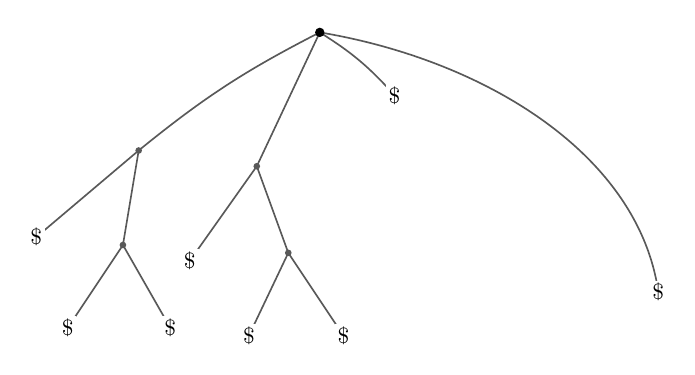
\begin{tikzpicture}[
    x=1cm,y=1cm,
    arco/.style={draw=black!65,line width=0.6pt},
    interno/.style={circle,fill=black!65,inner sep=0pt,minimum size=2.4pt},
    radice/.style={circle,fill=black,inner sep=0pt,minimum size=3.4pt},
    foglia/.style={inner sep=1pt,fill=white,font=\footnotesize}]

  % ---- coordinate ------------------------------------------------------
  \coordinate (r)   at ( 0.00, 0.00);   % radice

  \coordinate (la)  at ( 0.95,-0.80);   % foglia del suffisso "$"
  \coordinate (lb)  at ( 4.30,-3.30);   % foglia del suffisso piu' lungo (tutta T$)

  \coordinate (v1)  at (-2.30,-1.50);
  \coordinate (lc1) at (-3.60,-2.60);
  \coordinate (v1p) at (-2.50,-2.70);
  \coordinate (lc2) at (-3.20,-3.75);
  \coordinate (lc3) at (-1.90,-3.75);

  \coordinate (v2)  at (-0.80,-1.70);
  \coordinate (ld1) at (-1.65,-2.90);
  \coordinate (v2p) at (-0.40,-2.80);
  \coordinate (ld2) at (-0.90,-3.85);
  \coordinate (ld3) at ( 0.30,-3.85);

  % ---- archi -----------------------------------------------------------
  % (a) arco cortissimo: il suffisso costituito dalla sola sentinella
  \draw[arco] (r) to[bend left=8] (la);

  % (b) arco lunghissimo e curvo: il suffisso piu' lungo, ovvero tutto T$
  \draw[arco] (r) .. controls (2.10,-0.35) and (4.05,-1.55) .. (lb);

  % (c) ramo sinistro
  \draw[arco] (r) to[bend right=6] (v1);
  \draw[arco] (v1) -- (lc1);
  \draw[arco] (v1) -- (v1p);
  \draw[arco] (v1p) -- (lc2);
  \draw[arco] (v1p) -- (lc3);

  % (d) ramo centrale
  \draw[arco] (r) -- (v2);
  \draw[arco] (v2) -- (ld1);
  \draw[arco] (v2) -- (v2p);
  \draw[arco] (v2p) -- (ld2);
  \draw[arco] (v2p) -- (ld3);

  % ---- nodi ------------------------------------------------------------
  \node[radice]  at (r)   {};
  \node[interno] at (v1)  {};
  \node[interno] at (v1p) {};
  \node[interno] at (v2)  {};
  \node[interno] at (v2p) {};

  % ---- foglie: tutte marcate con la sentinella -------------------------
  \foreach \f in {la,lb,lc1,lc2,lc3,ld1,ld2,ld3}
    \node[foglia] at (\f) {$\$$};

\end{tikzpicture}

\caption{Il keyword tree dei suffissi di $T\$$ (suffix trie): ogni foglia corrisponde a un
suffisso e porta la sentinella $\$$.}
\label{fig:kwtree-suffissi}
\end{figure}

Se ho il keyword tree dei suffissi a disposizione, mi basta visitarlo e cercare il nodo
branching di profondità massima. Scriviamo $\cammino{v}$ per l'etichetta del cammino dalla
radice al nodo $v$, cioè per la stringa che quel cammino compita.

\begin{proposizione}[Sottostringa ripetuta più lunga]\label{prop:ripetuta}
\scan{17}
Sia $v$ un nodo branching di profondità massima del suffix trie di $T\$$. Allora
$\cammino{v}$ è la più lunga sottostringa ripetuta di $T$.
\end{proposizione}

\begin{dimostrazione}
Se $v$ è un nodo branching, ha almeno due figli e quindi almeno due foglie nel suo
sottoalbero, cioè almeno due suffissi distinti di cui $\cammino{v}$ è prefisso comune:
$\cammino{v}$ occorre allora in (almeno) due posizioni distinte di $T$, ed è ripetuta.
Viceversa, se $\b$ occorre in due posizioni distinte $i \neq j$, allora $\b$ è prefisso sia
del suffisso che comincia in $i$ sia di quello che comincia in $j$: i due cammini che dalla
radice compitano questi due suffissi condividono i primi $\abs{\b}$ archi e prima o poi si
separano, e il nodo in cui si separano è branching e ha profondità almeno $\abs{\b}$.
Massimizzare $\abs{\b}$ equivale dunque a massimizzare la profondità di un nodo branching.
La corrispondenza «nodi branching $\leftrightarrow$ sottostringhe ripetute» è esatta proprio
perché si lavora su $T\$$: con la sentinella ogni suffisso finisce in una foglia distinta,
mentre senza di essa un suffisso può essere prefisso di un altro (si pensi a $T = aa$) e la
sottostringa ripetuta $a$ non corrisponderebbe ad alcun nodo branching.
\end{dimostrazione}

Restano aperte due domande, che occupano il resto del capitolo:
\begin{enumerate}
  \item quanto è grande il keyword tree dei suffissi di $T$?
  \item come lo costruisco?
\end{enumerate}

\section{Notazione, definizione e dimensione del suffix trie}

\paragraph{Notazione.}
Il testo è $T = t_1 t_2 \cdots t_n$, di lunghezza $n = \abs{T}$, sull'alfabeto $\S$. Per ogni
$i \in \set{1,\dots,n}$ poniamo
\begin{align*}
  T^{\,i} &= \sub{T}{1}{i} = t_1 t_2 \cdots t_i,
          & &\text{$i$-esimo \emph{prefisso} di $T$},\\
  T_{i}   &= \sub{T}{i}{n} = t_i t_{i+1} \cdots t_n,
          & &\text{$i$-esimo \emph{suffisso} di $T$},
\end{align*}
con la convenzione $T^{\,0} = \vuota$, e indichiamo con
\[
  \mathcal{S}(T) \;=\; \set{\, T_i \;:\; i \in \set{1,\dots,n} \,}
\]
l'insieme di tutti i suffissi di $T$.

\begin{definizione}[Suffix trie]\label{def:strie}
Il \emph{suffix trie} di $T$ è il keyword tree dell'insieme dei suoi suffissi:
\[
  \STrie{}(T) \defeq K\bigl(\mathcal{S}(T)\bigr).
\]
\end{definizione}

Il termine \emph{trie}, per inciso, viene dall'inglese re\emph{trie}val.

Affrontiamo il primo dei due problemi.

\begin{domanda}
È possibile trovare esempi di $T$ tali che $\abs{\STrie{}(T)} \in \Th\bigl(\abs{T}^2\bigr)$?
\end{domanda}

Sì: basta prendere $T = a^m b^m$, e dunque $\abs{T} = 2m$.

\begin{figure}[H]
\centering
% Suffix trie di T = a^m b^m: spina dorsale di m archi 'a', da ogni suo nodo pende una
% catena di m archi 'b'  ==>  Theta(m^2) nodi.
\begin{tikzpicture}[
    x=0.95cm,y=0.95cm,
    arco/.style={draw=black,line width=0.5pt},
    nd/.style={circle,fill=black,inner sep=0pt,minimum size=2.6pt},
    rt/.style={circle,fill=black,inner sep=0pt,minimum size=3.8pt},
    et/.style={font=\scriptsize,inner sep=1.2pt},
    pnt/.style={circle,fill=black,inner sep=0pt,minimum size=1.5pt}]

  % =====================================================================
  % radice
  % =====================================================================
  \coordinate (r) at (0,0);

  % =====================================================================
  % catena dei suffissi b^q che pende dalla radice (verso destra-basso)
  % =====================================================================
  \coordinate (u1) at (0.85,-0.30);
  \coordinate (u2) at (1.70,-0.60);
  \coordinate (u3) at (2.55,-0.90);
  \draw[arco] (r)  -- (u1) node[et,midway,anchor=south]{$b$};
  \draw[arco] (u1) -- (u2) node[et,midway,anchor=south]{$b$};
  \draw[arco] (u2) -- (u3) node[et,midway,anchor=south]{$b$};
  \foreach \k in {1,2,3} \node[pnt] at ($(u3)+\k*(0.28,-0.10)$) {};
  \node[nd] at (u1) {}; \node[nd] at (u2) {}; \node[nd] at (u3) {};

  % =====================================================================
  % spina dorsale degli a (quasi verticale, m archi in tutto)
  % =====================================================================
  \coordinate (v1) at (-0.22,-0.95);
  \coordinate (v2) at (-0.44,-1.90);
  \coordinate (v3) at (-0.66,-2.85);
  \coordinate (v4) at (-0.88,-3.80);
  \coordinate (vm) at (-1.15,-5.35);

  \draw[arco] (r)  -- (v1) node[et,midway,anchor=east,xshift=-1pt]{$a$};
  \draw[arco] (v1) -- (v2) node[et,midway,anchor=east,xshift=-1pt]{$a$};
  \draw[arco] (v2) -- (v3) node[et,midway,anchor=east,xshift=-1pt]{$a$};
  \draw[arco] (v3) -- (v4) node[et,midway,anchor=east,xshift=-1pt]{$a$};
  % ellissi verticale sulla spina
  \draw[arco] (v4) -- (-0.93,-4.05);
  \foreach \k in {1,2,3} \node[pnt] at ($(-0.93,-4.05)+\k*(-0.045,-0.27)$) {};
  \draw[arco] (-1.09,-5.10) -- (vm);

  \node[nd] at (v1) {}; \node[nd] at (v2) {}; \node[nd] at (v3) {};
  \node[nd] at (v4) {}; \node[nd] at (vm) {};
  \node[rt] at (r) {};

  % =====================================================================
  % catene di b pendenti da ciascun nodo della spina (a 45 gradi)
  % di ognuna si disegnano i primi due archi, poi l'ellissi
  % =====================================================================
  \foreach \v in {v1,v2,v3,v4}{%
    \coordinate (p1) at ($(\v)+(0.62,-0.62)$);
    \coordinate (p2) at ($(\v)+(1.24,-1.24)$);
    \draw[arco] (\v) -- (p1) node[et,midway,anchor=south west]{$b$};
    \draw[arco] (p1) -- (p2) node[et,midway,anchor=south west]{$b$};
    \node[nd] at (p1) {}; \node[nd] at (p2) {};
    \foreach \k in {1,2,3} \node[pnt] at ($(p2)+\k*(0.24,-0.24)$) {};
  }

  % =====================================================================
  % ultima catena, quella appesa a v_m: compita l'intera stringa a^m b^m
  % =====================================================================
  \coordinate (w1) at (-0.93,-5.97);
  \coordinate (w2) at (-0.71,-6.59);
  \coordinate (w3) at (-0.49,-7.21);
  \draw[arco] (vm) -- (w1) node[et,midway,anchor=west]{$b$};
  \draw[arco] (w1) -- (w2) node[et,midway,anchor=west]{$b$};
  \draw[arco] (w2) -- (w3) node[et,midway,anchor=west]{$b$};
  \node[nd] at (w1) {}; \node[nd] at (w2) {}; \node[nd] at (w3) {};
  \foreach \k in {1,2,3} \node[pnt] at ($(w3)+\k*(0.09,-0.26)$) {};

  % =====================================================================
  % graffe di misura
  % =====================================================================
  % la spina e' fatta di m archi 'a'
  \draw[decorate,decoration={brace,amplitude=5pt}] (-1.75,-5.25) -- (-1.75,0);
  \node[font=\small] at (-2.20,-2.62) {$m$};
  % l'ultima catena e' fatta di m archi 'b'
  \draw[decorate,decoration={brace,amplitude=5pt}] (-1.75,-7.30) -- (-1.75,-5.55);
  \node[font=\small] at (-2.20,-6.42) {$m$};

\end{tikzpicture}

\caption{Il suffix trie di $T = a^m b^m$. La «spina dorsale» degli $a$ è lunga $m$ e da
ciascuno dei suoi nodi pende una catena di $m$ archi etichettati $b$: in tutto
$\Th(m^2) = \Th(\abs{T}^2)$ nodi.}
\label{fig:suffix-trie-ambm}
\end{figure}

Le sottostringhe di $a^m b^m$ sono infatti tutte e sole le stringhe della forma $a^p b^q$ con
$0 \le p \le m$ e $0 \le q \le m$, a due a due distinte; poiché i nodi del suffix trie di $T$
sono in biiezione con le sottostringhe distinte di $T$ --- ogni nodo è individuato dalla
stringa che il cammino dalla radice compita, e tali stringhe sono esattamente i prefissi dei
suffissi di $T$, cioè le sottostringhe di $T$ (alla radice corrisponde la stringa vuota
$\vuota$) --- il suffix trie di $T$ ha esattamente
\[
  (m+1)^2 \;=\; \frac{\abs{T}^2}{4} + \abs{T} + 1 \;=\; \Th\bigl(\abs{T}^2\bigr)
\]
nodi. Nel disegno: dalla radice pende la catena dei suffissi $b^q$, lunga $m$, e da ciascuno
dei nodi $a^p$ della spina dorsale degli $a$ pende una catena di $m$ archi etichettati $b$,
la cui foglia rappresenta il suffisso $a^p b^m$.

Il suffix trie è dunque inutilizzabile come indice: lo spazio è quadratico. È questa la
motivazione della compattazione che segue.

\section{Dal suffix trie al suffix tree}

\scan{18}
Guardiamo da vicino un frammento di suffix trie: lungo i rami si formano catene di nodi con
un solo figlio, ed è la proliferazione di questi nodi a rendere quadratica la dimensione
della struttura. L'idea è contrarre ogni catena in un unico arco, etichettato dalla stringa
che la catena compita: nel disegno, \str{abb}.

\begin{figure}[H]
\centering
% Contrazione di una catena unaria in un frammento di suffix trie:
% i nodi v1, v2 (un solo figlio) spariscono e il cammino abb diventa un unico arco [k,p].
\begin{tikzpicture}[
    x=0.92cm,y=0.92cm,
    arco/.style={draw=black,line width=0.5pt},
    nd/.style={circle,fill=black,inner sep=0pt,minimum size=2.8pt},
    ndg/.style={circle,fill=black,inner sep=0pt,minimum size=3.6pt},
    vuoto/.style={circle,draw=black,fill=white,line width=0.5pt,
                  inner sep=0pt,minimum size=4pt},
    et/.style={font=\footnotesize,inner sep=1.5pt},
    ann/.style={draw=accent,line width=1.1pt}]

  % =====================================================================
  % LIVELLO A -- il frammento di trie
  % =====================================================================
  \coordinate (u)  at ( 0.00, 0.00);
  \coordinate (x)  at (-1.30,-1.20);   % altro figlio di u (non interessa)
  \coordinate (v1) at ( 1.15,-1.15);
  \coordinate (v2) at ( 2.30,-2.30);
  \coordinate (w)  at ( 3.45,-3.45);
  \coordinate (f1) at ( 2.85,-4.55);
  \coordinate (f2) at ( 4.15,-4.55);

  % l'albero prosegue verso la radice
  \draw[arco] (0,1.90)
      .. controls ( 0.22, 1.72) and (-0.22, 1.56) .. (0,1.40)
      .. controls ( 0.22, 1.22) and (-0.22, 1.06) .. (0,0.90)
      .. controls ( 0.22, 0.72) and (-0.22, 0.56) .. (0,0.40)
      -- (u);

  \draw[arco] (u)  -- (x);
  \draw[arco] (u)  -- (v1) node[et,midway,anchor=south west]{$a$};
  \draw[arco] (v1) -- (v2) node[et,midway,anchor=south west]{$b$};
  \draw[arco] (v2) -- (w)  node[et,midway,anchor=south west]{$b$};
  \draw[arco] (w)  -- (f1);
  \draw[arco] (w)  -- (f2);

  \node[ndg] at (u)  {};
  \node[vuoto] at (x) {};
  \node[nd] at (v1) {};
  \node[nd] at (v2) {};
  \node[ndg] at (w)  {};
  \node[nd] at (f1) {};
  \node[nd] at (f2) {};

  % =====================================================================
  % LIVELLO B -- l'annotazione della compattazione
  % =====================================================================
  % cancellatura dei due nodi con un solo figlio
  \foreach \v in {v1,v2}{%
    \draw[ann] ($(\v)+(-0.38,-0.13)$) -- ($(\v)+(0.38,0.13)$);
    \draw[ann] ($(\v)+(-0.20,0.32)$)  -- ($(\v)+(0.20,-0.32)$);
  }

  % nuovo arco compattato u --> w, che scavalca la catena passando a sinistra
  \draw[ann] (u) .. controls (-0.90,-1.80) and (1.20,-4.30) .. (w);

  % etichetta dell'arco compattato
  \node[accent,align=center,anchor=east,font=\footnotesize] at (-0.35,-2.55)
        {\str{abb}\\[1pt]$[k,p]$};

\end{tikzpicture}

\caption{Contrazione di una catena unaria in un frammento di suffix trie: i due nodi
con un solo figlio vengono cancellati e il cammino \str{abb} diventa un unico arco, che verrà
etichettato con la coppia di indici $[k,p]$.}
\label{fig:compattazione-abb}
\end{figure}

Per garantire la linearità della struttura dati modifichiamo dunque il suffix trie in
\emph{suffix tree}. Servono due operazioni.

\paragraph{1) Eliminazione dei cammini unari.}
Eliminiamo i cammini massimali di nodi con un solo figlio: se
\[
  x_1 \xrightarrow{\;a_1\;} x_2 \xrightarrow{\;a_2\;} \cdots
       \xrightarrow{\;a_{h-1}\;} x_h
\]
è un cammino i cui nodi interni $x_2,\dots,x_{h-1}$ hanno esattamente un figlio, ed è
massimale (né $x_1$ né $x_h$ sono nodi unari), lo sostituiamo con il solo arco $(x_1,x_h)$.

\begin{figure}[H]
\centering
\begin{tikzpicture}[
    x=1cm, y=1cm, font=\footnotesize,
    vuoto/.style={circle,draw=black,line width=0.5pt,inner sep=0pt,minimum size=4.5pt},
    pieno/.style={circle,fill=black,inner sep=0pt,minimum size=3.6pt},
    arco/.style={-{Latex[length=4.5pt,width=3.2pt]},line width=0.6pt,
                 shorten >=2pt,shorten <=2pt}]

  %% ---------- pannello sinistro: la catena unaria x_1 ... x_h ----------
  \node[vuoto] (x1) at (0    , 0    ) {};
  \node[pieno] (x2) at (1    ,-0.95 ) {};
  \node[pieno] (x3) at (2    ,-1.90 ) {};
  \node[pieno] (xm) at (3.2  ,-3.04 ) {};
  \node[vuoto] (xh) at (4.2  ,-3.99 ) {};

  \draw[arco] (x1) -- node[left=1pt] {$a_1$}     (x2);
  \draw[arco] (x2) -- node[left=1pt] {$a_2$}     (x3);
  \draw[arco] (xm) -- node[left=1pt] {$a_{h-1}$} (xh);

  % i nodi omessi: tre puntini allineati sulla stessa diagonale
  \fill (2.36,-2.242) circle (0.7pt);
  \fill (2.60,-2.470) circle (0.7pt);
  \fill (2.84,-2.698) circle (0.7pt);

  \node[above right=-2pt] at (x1) {$x_1$};
  \node[right=2pt]        at (x2) {$x_2$};
  \node[right=2pt]        at (x3) {$x_3$};
  \node[right=2pt]        at (xm) {$x_{h-1}$};
  \node[right=2pt]        at (xh) {$x_h$};

  %% ---------- separatore ----------
  \draw[line width=0.45pt,double distance=1.5pt,-{Implies[length=4pt,width=5pt]}]
        (5.35,-2.0) -- (6.75,-2.0);

  %% ---------- pannello destro: l'unico arco (x_1,x_h) ----------
  \node[vuoto] (y1) at (7.6 ,-1.10) {};
  \node[vuoto] (yh) at (8.8 ,-2.24) {};
  \draw[arco] (y1) -- (yh);

  \node[above right=-2pt] at (y1) {$x_1$};
  \node[right=2pt]        at (yh) {$x_h$};

\end{tikzpicture}

\caption{Operazione 1: la catena massimale di nodi con un solo figlio $x_1,\dots,x_h$ viene
sostituita dall'unico arco $(x_1,x_h)$.}
\label{fig:compattazione-catena}
\end{figure}

\paragraph{2) Etichette come coppie di indici.}
Etichetto l'arco $(x_1,x_h)$ così introdotto con una coppia $[k,p]$ di indici nel testo tale
che
\[
  \sub{T}{k}{p} \;=\; a_1 a_2 \cdots a_{h-1}.
\]

\begin{osservazione}
Di coppie $[k,p]$ che individuano quella sottostringa ce ne può essere più d'una --- tante
quante le occorrenze di $a_1 a_2 \cdots a_{h-1}$ in $T$ --- e la scelta fra esse è del tutto
indifferente: quel che conta è la stringa compitata, non la posizione da cui la si legge.
\end{osservazione}

\begin{osservazione}
Affinché 2) funzioni dobbiamo tenere in memoria anche il testo: l'etichetta non contiene più
i caratteri, ma soltanto un puntatore alla porzione di $T$ che li contiene. La struttura dati
finale è dunque il trie compattato \emph{più} il testo $T$.
\end{osservazione}

\subsection{Linearità}

\begin{lemma}[Alberi con soli nodi branching]\label{lem:branching}
Sia $\T$ un albero finito con $\ell$ foglie e $I$ nodi interni, in cui ogni nodo interno è
\emph{branching}, cioè ha almeno due figli. Allora
\[
  I \;\le\; \ell - 1,
  \qquad\text{e dunque}\qquad
  I + \ell \;\le\; 2\ell - 1 ,
\]
cioè $\T$ ha al più $2\ell-1$ nodi. Vale l'uguaglianza se e solo se ogni nodo interno ha
esattamente due figli, cioè se e solo se $\T$ è binario.
\end{lemma}

\begin{dimostrazione}
In un albero gli archi sono $I + \ell - 1$ (uno per nodo, tranne la radice); d'altra parte
ogni arco esce da esattamente un nodo interno e ogni nodo interno ha almeno due archi
uscenti, dunque
\[
  I + \ell - 1 \;=\; \sum_{u \text{ interno}} \deg^{+}(u) \;\ge\; 2I ,
  \qquad\text{cioè}\qquad I \;\le\; \ell - 1 .
\]
Sommando le foglie, il numero di nodi è $I + \ell \le 2\ell - 1$. L'uguaglianza vale
esattamente quando $\deg^{+}(u) = 2$ per ogni nodo interno $u$.
\end{dimostrazione}

\begin{figure}[H]
\centering
% Il lemma "ogni nodo interno e' branching" a colpo d'occhio.
% Stesso albero (4 foglie, 3 nodi interni) disegnato due volte:
%  a sinistra l'addebito nodo interno -> foglia, a destra la contrazione di una ciliegia.
\begin{tikzpicture}[
    x=1cm, y=1cm, font=\footnotesize,
    arco/.style={draw=black,line width=0.5pt},
    nodo/.style={circle,draw=black,fill=white,line width=0.5pt,
                 inner sep=0pt,minimum size=4.5pt},
    addebito/.style={draw=graydark,line width=0.5pt,densely dashed,
                     -{Latex[length=4pt,width=3pt]}}]

  %% ===================================================================
  %% PANNELLO SINISTRO -- ogni nodo interno addebitato a una foglia
  %% ===================================================================
  \begin{scope}[shift={(0,0)}]
    \coordinate (r)  at (1.50, 2.00);
    \coordinate (u)  at (0.75, 1.00);
    \coordinate (w)  at (2.25, 1.00);
    \coordinate (f1) at (0.25, 0.00);
    \coordinate (f2) at (1.25, 0.00);
    \coordinate (f3) at (1.75, 0.00);
    \coordinate (f4) at (2.75, 0.00);

    \draw[arco] (r) -- (u);  \draw[arco] (r) -- (w);
    \draw[arco] (u) -- (f1); \draw[arco] (u) -- (f2);
    \draw[arco] (w) -- (f3); \draw[arco] (w) -- (f4);

    % l'addebito: da ogni nodo interno si scende a una foglia del suo sottoalbero
    \draw[addebito] (1.50,1.82) -- (1.50,-0.30);
    \draw[addebito] (0.75,0.82) -- (0.75,-0.30);
    \draw[addebito] (2.25,0.82) -- (2.25,-0.30);

    \foreach \n in {r,u,w,f1,f2,f3,f4} \node[nodo] at (\n) {};

    \node[anchor=north,align=center] at (1.50,-0.62)
          {addebito nodo interno $\to$ foglia\\[1pt] $I \le \ell$};
  \end{scope}

  %% ===================================================================
  %% PANNELLO DESTRO -- contrazione di una ciliegia
  %% ===================================================================
  \begin{scope}[shift={(5.60,0)}]
    \coordinate (R)  at (1.50, 2.00);
    \coordinate (U)  at (0.75, 1.00);
    \coordinate (W)  at (2.25, 1.00);
    \coordinate (g1) at (0.25, 0.00);
    \coordinate (g2) at (1.25, 0.00);
    \coordinate (g3) at (1.75, 0.00);
    \coordinate (g4) at (2.75, 0.00);

    \draw[arco] (R) -- (U);  \draw[arco] (R) -- (W);
    \draw[arco] (U) -- (g1); \draw[arco] (U) -- (g2);
    \draw[arco] (W) -- (g3); \draw[arco] (W) -- (g4);

    % la ciliegia: nodo branching i cui figli sono tutte foglie
    \draw[draw=accent,line width=1.1pt]
      plot[smooth cycle,tension=0.75] coordinates
      {(0.75,1.40) (1.36,0.52) (1.42,-0.34) (0.06,-0.42) (-0.20,0.45)};

    \foreach \n in {R,U,W,g1,g2,g3,g4} \node[nodo] at (\n) {};

    \node[anchor=north,align=center] at (1.50,-0.62)
          {contrazione di una ciliegia\\[1pt] $(I,\ell) \to (I-1,\ell-1)$};
  \end{scope}

\end{tikzpicture}

\caption{Il Lemma a colpo d'occhio, su un albero con $4$ foglie e $3$ nodi interni
($7 = 2\cdot 4 - 1$ nodi). A sinistra: ogni nodo interno viene addebitato a una foglia
distinta del proprio sottoalbero, da cui $I \le \ell$. A destra: la contrazione di una
\emph{ciliegia} (nodo branching i cui figli sono tutti foglie, cerchiata) toglie un nodo
interno e una foglia, e permette di concludere per induzione.}
\label{fig:lemma-branching}
\end{figure}

Il Lemma, insieme alle operazioni 1) e 2), garantisce la linearità del suffix tree. Dopo la
compattazione, infatti, ogni nodo interno è branching e le foglie sono una per suffisso,
cioè $n+1$ lavorando su $T\$$ e comunque $\Oh(n)$; quindi
\[
  \#\text{nodi} \;\le\; 2(n+1) - 1 \;=\; \Oh(n),
\]
gli archi sono uno di meno, e ciascuno di essi porta due soli interi. Sommando il testo, che
va comunque tenuto in memoria, lo spazio complessivo è $\Oh(n)$.

\section{A che cosa serve il suffix tree}

\scan{19}
Una volta costruito l'albero dei suffissi del testo, la ricerca di un pattern $P$ si riduce a
compitare $P$ lungo l'unico cammino che parte dalla radice: se il cammino esiste e termina
nel nodo (eventualmente implicito) $v$, le foglie del sottoalbero $\albero{v}$ radicato in
$v$ sono esattamente le occorrenze di $P$ in $T$.

\begin{figure}[H]
\centering
% Ricerca esatta col suffix tree: si compita P dalla radice, si arriva al nodo v,
% e le foglie del sottoalbero T(v) sono le occorrenze di P in T.
% La "montagna" e' il suffix tree dell'intero testo, disegnato come sagoma.
\begin{tikzpicture}[
    x=0.86cm, y=0.86cm, font=\footnotesize,
    profilo/.style={draw=black,line width=0.7pt,line join=round},
    sotto/.style={draw=black,line width=0.4pt,line join=round},
    barra/.style={draw=black,line width=1.1pt,line cap=round},
    foglia/.style={circle,fill=black,inner sep=0pt,minimum size=3.2pt}]

  %% ===================================================================
  %% 1) promemoria: P e' corto, T e' lungo
  %% ===================================================================
  \draw[barra] (0.90,2.55) -- (2.10,2.55);
  \draw[barra] (0.90,1.80) -- (4.10,1.80);
  \node[anchor=south west,inner sep=1pt] at (0.90,2.61) {$P$};
  \node[anchor=south west,inner sep=1pt] at (0.90,1.86) {$T$};

  %% ===================================================================
  %% 2) la montagna: l'intero suffix tree di T
  %% ===================================================================
  \draw[profilo]                                  % versante sinistro
     (7.50, 3.40) -- (7.15, 2.95) -- (7.05, 2.60) -- (6.58, 2.10)
  -- (6.45, 1.70) -- (5.99, 1.20) -- (5.85, 0.80) -- (5.40, 0.30)
  -- (5.25,-0.10) -- (4.81,-0.60) -- (4.65,-1.00) -- (4.32,-1.35)
  -- (4.20,-1.60);
  \draw[profilo]                                  % versante destro
     (7.50, 3.40) -- (7.85, 2.95) -- (7.95, 2.60) -- (8.42, 2.10)
  -- (8.55, 1.70) -- (9.01, 1.20) -- (9.15, 0.80) -- (9.60, 0.30)
  -- (9.75,-0.10) -- (10.19,-0.60) -- (10.35,-1.00) -- (10.68,-1.35)
  -- (10.80,-1.60);
  \draw[draw=graylight,line width=0.4pt] (4.20,-1.60) -- (10.80,-1.60);

  % la radice, in cima
  \node[foglia] at (7.50,3.40) {};
  \node[anchor=south,inner sep=2pt] at (7.50,3.44) {radice};

  %% ===================================================================
  %% 3) il cammino che compita P, dalla radice fino a v
  %% ===================================================================
  \draw[draw=black,line width=1.1pt,line join=round]
     (7.50,3.40) -- (7.44,2.90) -- (7.53,2.45) -- (7.38,1.95)
  -- (7.48,1.45) -- (7.40,0.90);
  \node[anchor=west,inner sep=2pt,font=\normalsize] at (7.62,2.20) {$P$};

  %% ===================================================================
  %% 4) il nodo v e il sottoalbero T(v) che vi e' appeso
  %% ===================================================================
  \draw[sotto]
     (7.40,0.90) -- (7.15,0.35) -- (7.22,0.00) -- (6.72,-0.60)
  -- (6.62,-1.00) -- (6.00,-1.40);
  \draw[sotto]
     (7.40,0.90) -- (7.68,0.40) -- (7.62,0.00) -- (8.12,-0.55)
  -- (8.22,-0.95) -- (8.90,-1.40);
  % base del sottoalbero: linea ondulata, su cui stanno le foglie
  \draw[sotto,decorate,decoration={snake,amplitude=0.6mm,segment length=5mm}]
     (6.00,-1.40) -- (8.90,-1.40);

  \node[foglia] at (6.55,-1.40) {};
  \node[foglia] at (8.30,-1.40) {};

  \node[circle,fill=black,inner sep=0pt,minimum size=4pt] at (7.40,0.90) {};
  \node[anchor=east,inner sep=3pt] at (7.40,0.90) {$v$};

  \node[anchor=west,inner sep=1pt] (etv) at (9.10,-0.62) {$\albero{v}$};
  \draw[-{Latex[length=3.5pt,width=2.5pt]},line width=0.4pt]
        (etv.west) -- (8.45,-0.88);

  \node[anchor=north,text=graydark] at (7.45,-1.95)
        {occorrenze di $P$ in $T$};

\end{tikzpicture}

\caption{Uso del suffix tree per la ricerca esatta: il cammino che compita $P$ dalla radice
termina nel nodo $v$; le foglie del sottoalbero $\albero{v}$ appeso a $v$ sono le occorrenze
di $P$ in $T$.}
\label{fig:suffix-tree-ricerca-montagna}
\end{figure}

\begin{osservazione}
A lato del disegno gli appunti richiamano Boyer--Moore («e anche Boyer--Moore»), senza
ulteriori dettagli.
\end{osservazione}

\section{L'algoritmo di Ukkonen}

\scan{19}
\begin{domanda}
Come costruisco il suffix tree?
\end{domanda}

\begin{osservazione}
Soluzioni al problema esistono già dagli anni Settanta --- Weiner (1973) e McCreight (1976)
--- ma quella di Ukkonen è molto più chiara ed è quella che tutti citano.
\end{osservazione}

L'algoritmo di Ukkonen (1995), presentato nell'articolo \emph{On-line construction of suffix
trees}, è \emph{on-line} sul testo $T = t_1 t_2 \cdots t_n$: ne legge un carattere alla volta,
da sinistra a destra, e mantiene in ogni istante la struttura relativa al prefisso già letto.
Il passo generico trasforma la struttura del prefisso $T^{\,i-1}$ in quella del prefisso
$T^{\,i}$ leggendo il carattere $t_i$:
\[
  \STrie{}(T^{\,i-1}) \;\xrightarrow{\ t_i\ }\; \STrie{}(T^{\,i}).
\]

\begin{figure}[H]
\centering
% Un passo di Ukkonen: dal prefisso T^{i-1} (gia' processato) a T^i, leggendo t_i.
% La riga superiore ricorda un generico suffisso T_j che attraversa il passo.
\begin{tikzpicture}[
    x=0.84cm, y=0.84cm, font=\small,
    testo/.style={draw=black,line width=1.1pt,line cap=round},
    tacca/.style={draw=black,line width=0.5pt,line cap=round}]

  % la cella del carattere corrente t_i, sullo sfondo
  \fill[black!14] (5.40,-0.10) rectangle (5.90,0.55);

  %% ---------------- le due barre --------------------------------------
  \draw[testo] (0,0)    -- (12,0);       % il testo T
  \draw[testo] (3,0.45) -- (12,0.45);    % il suffisso T_j
  \node[anchor=west,inner sep=4pt] at (12,0) {$T$};

  %% ---------------- tacche --------------------------------------------
  \draw[tacca] (0,-0.20) -- (0,0.25);                    % inizio del testo
  \draw[tacca] (3,-0.28) -- (3,0.66);                    % posizione j
  \draw[tacca] (5.40,-0.30) -- (5.40,1.00);              % coppia che
  \draw[tacca] (5.90,-0.30) -- (5.90,1.00);              % isola t_i

  \node[anchor=south,inner sep=2pt] at (3,0.68) {$T_j$};
  \node[anchor=north,inner sep=2pt] at (3,-0.30) {$j$};

  \node[anchor=west,inner sep=1pt] (lti) at (6.55,1.28) {$t_i$};
  \draw[-{Latex[length=4pt,width=3pt]},line width=0.5pt]
        (lti.west) -- (5.66,1.06);

  %% ---------------- graffa sul prefisso gia' letto ---------------------
  \draw[line width=0.5pt,decorate,decoration={brace,mirror,amplitude=5pt}]
        (0,-0.95) -- (5.40,-0.95);

  % collegamento fra la tacca in i e la riga in basso
  \draw[draw=graylight,line width=0.4pt,densely dashed]
        (5.40,-0.34) -- (5.40,-1.72);

  %% ---------------- la riga del passo ---------------------------------
  \node[anchor=center] at (2.70,-1.95) {$\STrie{}(T^{\,i-1})$};
  \draw[-{Latex[length=4.5pt,width=3.2pt]},line width=0.5pt]
        (5.20,-1.95) -- (6.40,-1.95);
  \node[anchor=south,inner sep=2pt] at (5.80,-1.88) {$t_i$};
  \node[anchor=west] at (6.60,-1.95) {$\STrie{}(T^{\,i})$};

\end{tikzpicture}

\caption{Un passo dell'algoritmo di Ukkonen. Il prefisso $T^{\,i-1}$ è già stato processato;
leggendo il carattere $t_i$ si passa a $\STrie{}(T^{\,i})$. La riga superiore evidenzia un
generico suffisso $T_j$, che nel passo corrente contribuisce con la sua parte
$t_j \cdots t_{i-1}$.}
\label{fig:ukkonen-passo-prefissi}
\end{figure}

La strategia viene esposta in due tempi:
\begin{itemize}
  \item[(a)] si illustra la strategia nel caso dei \emph{suffix trie};
  \item[(b)] si modifica la strategia e la si adatta ai \emph{suffix tree}.
\end{itemize}
In entrambi i casi la struttura su cui si lavora è la versione \emph{aumentata}
(\emph{augmented}) della struttura dati --- l'automa a stati finiti con lo stato ausiliario
$\bot$ e la funzione dei suffix link --- che definiamo subito.

Costruiremo dunque $\STrie{}(T^{\,i})$ per $i = 1,\dots,n$ --- \emph{in quest'ordine!} --- a
partire da $\STrie{}(T^{\,i-1})$, appendendo $t_i$ sotto ogni suffisso di $T^{\,i-1}$; il caso
base è $\STrie{}(T^{\,0})$, il trie della stringa vuota, cioè il solo nodo radice.

\subsection{Il suffix trie come automa aumentato}

\scan{20}
\begin{definizione}[Suffix trie come automa aumentato]\label{def:strie-automa}
Dato il testo $T$, il \emph{suffix trie} di $T$ è la quintupla
\[
  \STrie{}(T)\;=\;\bigl(\,Q\cup\set{\bot},\;\mathit{root},\;F,\;g,\;f\,\bigr),
\]
dove, scrivendo $\bar{x}$ per lo stato associato alla stringa $x$,
\begin{align*}
  Q             &= \set{\bar{x} \;:\; x \text{ sottostringa di } T}
                   &&\text{insieme degli stati,}\\
  \mathit{root} &= \bar{\vuota} &&\text{stato iniziale,}\\
  F             &= \set{\bar{x} \;:\; x \text{ suffisso di } T} &&\text{stati finali,}\\
  g(\bar{x},a)  &= \overline{xa} \ \text{ se } xa \text{ è sottostringa di } T
                   \ \text{(altrimenti indefinita)}, &&\text{funzione di transizione}\\
                &\phantom{{}={}} \qquad g(\bot,a)=\mathit{root}
                   \ \text{ per ogni } a\in\S &&\text{(parziale),}\\
  f(\bar{x})    &= \bar{y} \ \text{ se } x = a\,y \ (a\in\S),
                   \qquad f(\mathit{root}) = \bot &&\text{suffix link.}
\end{align*}
Gli stati sono dunque in corrispondenza biunivoca ($1{:}1$) con le sottostringhe di $T$ (alla
stringa vuota corrisponde $\mathit{root}$), mentre $\bot$ è uno stato «dummy» ausiliario.
\end{definizione}

Le prime quattro componenti, $\bigl(Q\cup\set{\bot},\mathit{root},F,g\bigr)$, sono quelle di
un automa a stati finiti deterministico (DFA), con la sola differenza che $g$ è
\emph{parziale}: da $\bar{x}$ non esce alcun arco etichettato $a$ quando $xa$ non compare in
$T$. È l'ultima componente $f$ a rendere la struttura un \emph{automa aumentato}
(\emph{augmented automaton}). I suffix tree che
vogliamo costruire sono, allo stesso modo, automi deterministici a stati finiti
\emph{aumentati} che accettano tutti e soli i suffissi di un testo.

\begin{osservazione}
Accanto alla riga di $F$ gli appunti annotano, con una freccia, la parola «necessario»: è $F$
a fare di $\STrie{}(T)$ un automa che riconosce \emph{esattamente} i suffissi di $T$, e non
semplicemente le sue sottostringhe.
\end{osservazione}

\scan{21}
Il suffix link $f$ porta dallo stato associato alla stringa $x$ allo stato associato alla
stringa che si ottiene da $x$ cancellandone il primo carattere; la clausola
$f(\mathit{root}) = \bot$ lo rende totale.

\subsection{Il boundary path}

\begin{osservazione}
La funzione $f$ mi consente di costruire un cammino che visita \emph{tutti} i suffissi di
$T$. Partendo dallo stato $\bar{x}$ associato al suffisso più lungo, $x = t_1 t_2 \cdots t_n
= T$, e applicando ripetutamente $f$ si ottiene
\[
  \overline{t_1\cdots t_n}
  \;\xrightarrow{\ f\ }\; \overline{t_2\cdots t_n}
  \;\xrightarrow{\ f\ }\; \cdots
  \;\xrightarrow{\ f\ }\; \overline{t_n}
  \;\xrightarrow{\ f\ }\; \mathit{root}
  \;\xrightarrow{\ f\ }\; \bot .
\]
Questo cammino prende il nome di \textbf{boundary path}.
\end{osservazione}

\begin{figure}[H]
\centering
% Boundary path di STrie(T).
% La "montagna" schematizza il trie: il vertice e' la radice, la linea ondulata
% in basso e' la frontiera degli stati piu' profondi.  Su di essa stanno gli
% stati dei suffissi di T, collegati fra loro dai suffix link f.
\begin{tikzpicture}[
    scale=1.15,
    >={Stealth[length=4.5pt]},
    font=\footnotesize,
    stato/.style={circle,fill,inner sep=0pt,minimum size=4.4pt}]

  % ---- contorno schematico dello STrie -------------------------------------
  \draw[gray]
    (0,3.0) -- (-0.45,2.55) -- (-0.85,2.42) -- (-1.35,1.62)
         -- (-1.70,1.42) -- (-2.05,0.62) -- (-2.30,0.10);
  \draw[gray]
    (0,3.0) -- (0.40,2.50) -- (0.85,2.40) -- (1.45,1.78)
         -- (1.90,1.70) -- (2.45,1.15) -- (2.80,0.85);
  % frontiera degli stati piu' profondi
  \draw[gray] plot[smooth,tension=0.85] coordinates
    {(-2.30,0.10) (-1.90,-0.05) (-1.50,0.18) (-1.05,-0.02) (-0.60,0.22)
     (-0.15,0.30) (0.30,0.58) (0.80,0.36) (1.20,0.44) (1.60,0.62)
     (2.05,0.86) (2.45,0.70) (2.80,0.85)};

  % ---- stati dei suffissi ---------------------------------------------------
  \node[stato] (x) at (-1.90,-0.05) {};
  \node[stato] (y) at (-0.15, 0.30) {};
  \node[stato] (z) at ( 1.60, 0.62) {};
  \node[below left=1pt and 0pt] at (x) {$\bar{x}$};
  \node[above left=-2pt and -4pt] at (y) {$\bar{y}$};

  % ---- suffix link ----------------------------------------------------------
  \draw[->,thick] (x) to[out=-55,in=-125]
        node[pos=0.28,below=-1pt] {$f$} (y);
  \draw[->,thick] (y) to[out=70,in=125] (z);

  % ---- etichette esterne ----------------------------------------------------
  \node[anchor=east,align=right] at (-3.55,0.80)
       {suffisso\\[1pt] $t_1\cdots t_n = x$};
  \draw[->,gray,decorate,
        decoration={snake,amplitude=.5mm,segment length=3.2mm,post length=2mm}]
       (-3.45,0.95) -- (-2.38,0.55);

  \node[anchor=north] at (0.75,-1.05) {suffisso $t_2\cdots t_n$};
  \draw[->,gray] (0.62,-0.95) to[out=140,in=-35] (y);

  \node[anchor=west] at (2.95,0.08) {suffisso $t_3\cdots t_n$};
  \draw[->,gray] (2.88,0.20) to[out=165,in=-20] (z);
\end{tikzpicture}

\caption{Il \emph{boundary path} di $\STrie{}(T)$: applicando ripetutamente il suffix link $f$
a partire dallo stato $\bar{x}$ del suffisso più lungo $x = t_1\cdots t_n$ si incontrano,
nell'ordine, gli stati di tutti i suffissi di $T$.}
\label{fig:boundary-path}
\end{figure}

\scan{22}
Il boundary path è ciò che definisce i nodi finali dello \STrie{}. Durante il passo che legge
$t_i$ il cammino che interessa è quello di $\STrie{}(T^{\,i-1})$: percorrendolo si incontrano,
nell'ordine, gli stati
\[
  s_j \;=\; \overline{t_j t_{j+1} \cdots t_{i-1}}
        \;=\; f^{\,j-1}\bigl(\overline{t_1\cdots t_{i-1}}\bigr),
  \qquad j = 1,\dots,i,
\]
cioè $s_1 = \mathit{top} = \overline{t_1\cdots t_{i-1}}$, poi $s_2 = \overline{t_2\cdots
t_{i-1}}$, e così via fino a $s_i = \overline{\vuota} = \mathit{root}$, seguito da $\bot$:
sono esattamente gli stati che rappresentano i suffissi di $T^{\,i-1}$, e per costruzione
$s_{j+1} = f(s_j)$.

\subsection{Costruzione del suffix trie}

\scan{21}
Passerò da $\STrie{}(T^{\,i-1})$ a $\STrie{}(T^{\,i})$ visitando il boundary path e
aggiungendo una transizione, quando necessario, ad ogni passo: a ogni nodo che vi si incontra
--- cioè a ogni nodo legato a un suffisso di $T^{\,i-1}$ --- appendo un nuovo nodo con un arco
etichettato $t_i$, \textbf{se} da quel nodo non escono già archi etichettati con $t_i$.

Il motivo per cui questo basta è che l'insieme degli stati cresce solo lungo i suffissi:
\[
  Q\bigl(T^{\,i}\bigr) \;=\; Q\bigl(T^{\,i-1}\bigr) \;\cup\;
  \set{\, \overline{t_j\cdots t_i} \;:\; 1 \le j \le i \,} .
\]
Infatti ogni sottostringa di $T^{\,i}$ che non sia già sottostringa di $T^{\,i-1}$ deve
terminare con il carattere $t_i$, cioè è un suffisso di $T^{\,i}$; e i suffissi di $T^{\,i}$
sono esattamente gli stati del boundary path di $\STrie{}(T^{\,i-1})$ estesi con $t_i$.

\begin{algorithm}[H]
\caption{Costruzione di $\STrie{}(T)$ per $T = t_1 t_2 \cdots t_n$ (Ukkonen, Algoritmo 1)}
\label{alg:ukkonen-trie}
\begin{algorithmic}[1]
  \State crea gli stati $\mathit{root}$ e $\bot$
  \State $g(\bot, a) \gets \mathit{root}$ per ogni $a \in \S$;\quad
         $f(\mathit{root}) \gets \bot$
  \State $\mathit{top} \gets \mathit{root}$
  \For{$i \gets 1$ \textbf{to} $n$}
    \State $r \gets \mathit{top}$
    \While{$g(r, t_i)$ è indefinita}
      \State crea un nuovo stato $r'$ e poni $g(r, t_i) \gets r'$
      \If{$r \neq \mathit{top}$}
        \State $f(\mathit{oldr}') \gets r'$
        \Comment{$\mathit{oldr}'$ appartiene ancora al passo precedente}
      \EndIf
      \State $\mathit{oldr}' \gets r'$
      \State $r \gets f(r)$
    \EndWhile
    \State $f(\mathit{oldr}') \gets g(r, t_i)$
    \State $\mathit{top} \gets g(\mathit{top}, t_i)$
  \EndFor
\end{algorithmic}
\end{algorithm}

\begin{osservazione}
Il ciclo \textbf{while} esegue sempre almeno un'iterazione, perché $\mathit{top}$ è lo stato
più profondo del trie e non ha archi uscenti; e termina sempre, perché risalendo il boundary
path con $r \gets f(r)$ si arriva al più a $\bot$, dove $g(\bot, t_i) = \mathit{root}$ è
definita per ogni carattere. La guardia $r \neq \mathit{top}$ serve a non sovrascrivere il
suffix link dell'ultimo stato creato al passo precedente: i suffix link vengono assegnati
all'indietro (allo stato creato subito dopo), e il primo stato creato nel passo $i$ --- il
figlio di $\mathit{top}$ --- non ha, in quel passo, alcun predecessore cui attaccarsi.
La variabile $\mathit{top}$ mantiene l'invariante
$\mathit{top} = \overline{t_1\cdots t_i}$ alla fine del passo $i$-esimo, cioè è sempre il capo
del boundary path corrente.
\end{osservazione}

\paragraph{Costo.}
Per costruire $\STrie{}(T)$ eseguo $n$ volte l'operazione
$\STrie{}(T^{\,i-1}) \longrightarrow \STrie{}(T^{\,i})$, e ognuna costa $\Oh(i)$: il boundary
path di $\STrie{}(T^{\,i-1})$ ha infatti $i$ stati (i suffissi di $T^{\,i-1}$, compresa
$\vuota$, cioè la radice) più lo stato $\bot$. Sommando,
\[
  \sum_{i=1}^{n} \Oh(i) \;=\; \Oh\bigl(\abs{T}^{2}\bigr),
\]
cioè un \textbf{algoritmo quadratico}. Ed è \emph{ottimo}: la sola dimensione di
$\STrie{}(T)$ può essere $\Th(\abs{T}^{2})$ --- si pensi a $T = a^m b^m$ --- quindi nessun
algoritmo che costruisca esplicitamente il suffix trie può costare meno.

\subsection[Il boundary path si può accorciare]{Non serve percorrere tutto il boundary path}

\scan{22}
\begin{osservazione}
\textbf{Non} è sempre necessario visitarlo tutto!
\end{osservazione}

Gli stati del boundary path rappresentano infatti suffissi via via più corti: se $\bar s$
possiede già una $t_i$-transizione, allora $s\,t_i$ occorre in $T^{\,i-1}$, e quindi anche
$s'\,t_i$ occorre in $T^{\,i-1}$ per ogni suffisso $s'$ di $s$. Tutti gli stati che seguono
$\bar s$ sul boundary path hanno perciò già la loro $t_i$-transizione, e il ciclo
\textbf{while} dell'Algoritmo~\ref{alg:ukkonen-trie} può fermarsi al primo nodo $r$ per cui
$g(r,t_i)$ è definita --- come in effetti fa.

Questo non cambia la complessità asintotica finché si costruisce il trie: l'algoritmo resta
quadratico per la sola ragione che già la dimensione di $\STrie{}(T)$ può essere
$\Th(\abs{T}^{2})$. È però l'osservazione su cui poggia tutto il guadagno del passaggio al
suffix tree.

\subsection[Dallo STrie allo STree: i due ingredienti]%
{Dallo \texorpdfstring{\STrie{}}{STrie} allo \texorpdfstring{\STree{}}{STree}: i due ingredienti}

Per passare dallo \STrie{} allo \STree{} servono \emph{due ingredienti}:
\begin{enumerate}
  \item[(i)] tenere i \emph{soli nodi branching};
  \item[(ii)] rimpiazzare le etichette-stringa con coppie di interi,
        $w \longrightarrow [k,p]$.
\end{enumerate}
Entrambi servono a limitare a $\Oh(\abs{T})$ la dimensione dello \STree{}.

\begin{domanda}
Come uso (i) e (ii) nella definizione e nella costruzione dello \STree{}?
\end{domanda}

\textbf{(i)} non è un problema: mi limiterò ai nodi branching e definirò le transizioni
\emph{su stringhe},
\[
  g'(\bar x,\,w) \;=\; \overline{xw},
\]
dove il secondo argomento $w$ non è più un singolo carattere ma una stringa, rappresentata
dalla coppia di interi $[k,p]$, cioè $w = \sub{T}{k}{p}$.

\subsection[Stati espliciti e impliciti]{Stati espliciti, stati impliciti e coppie di riferimento}

\scan{23}
\textbf{(ii)} Per costruire $\STree{}(T^{\,i})$ a partire da $\STree{}(T^{\,i-1})$ dovrò
\emph{reintrodurre stati}. Introduciamo perciò due tipi di stato:
\begin{itemize}
  \item stati \emph{espliciti} (\emph{tree}): i nodi branching --- e le foglie --- che
        sopravvivono nell'albero compattato;
  \item stati \emph{impliciti} (\emph{trie-only}): quelli che esistono nel trie ma non
        nell'albero, perché cadono all'interno di un arco compattato.
\end{itemize}

\begin{definizione}[Il suffix tree come automa]\label{def:stree-automa}
\[
  \STree{}(T) \;=\; \bigl(\, Q' \cup \set{\bot},\ \mathit{root},\ g',\ f' \,\bigr),
\]
dove $Q'$ è l'insieme degli stati espliciti, $g'$ la funzione di transizione su stringhe
appena definita e $f'$ la funzione dei suffix link ristretta a $Q'$.

Gli stati --- impliciti ed espliciti --- sono dati da \emph{reference pair} (coppie di
riferimento): coppie $(s,w)$ con $s$ stato esplicito e $w$ stringa, cioè, rappresentando $w$
con la coppia di interi, $\bigl(s,[k,p]\bigr)$.
\end{definizione}

\begin{osservazione}
Di $w$ interessa soltanto il \emph{primo carattere}: è quello che decide quale arco uscente da
$s$ imboccare. Se $t_k = a$ chiamiamo la transizione una \emph{$a$-transizione}.
\end{osservazione}

\begin{figure}[H]
\centering
% Due esempi di reference pair (s,w): stesso s, stringhe w di lunghezza diversa,
% quindi due stati impliciti distinti dello stesso arco.
% Il nodo pieno e' lo stato esplicito (branching) s; lungo l'arco lungo stanno
% gli stati impliciti (cerchietti vuoti); la graffa misura la stringa w.
\begin{tikzpicture}[
    scale=1.2,
    font=\footnotesize,
    esplicito/.style={circle,fill,inner sep=0pt,minimum size=5pt},
    implicito/.style={circle,draw,fill=white,inner sep=0pt,minimum size=4pt},
    graffa/.style={decorate,decoration={brace,amplitude=4pt},gray}]

  % il secondo schizzo e' identico al primo: cambia solo dove finisce la graffa
  \foreach \dx/\tfin/\lx/\ly in {0/0.42/0.87/-0.25, 3.6/0.82/1.13/-0.77}{%
    \begin{scope}[xshift=\dx cm]
      % l'altro figlio di s: s e' un branching point
      \draw (0,0) -- (-0.85,-0.85);
      % arco lungo, con gli stati impliciti che il trie ha e l'albero no
      \draw (0,0) -- (1.30,-2.60);
      \foreach \t in {0.22,0.42,0.62,0.82}
        \node[implicito] at ({1.30*\t},{-2.60*\t}) {};
      % stato esplicito
      \node[esplicito] at (0,0) {};
      \node[above left=-3pt and -3pt] at (0,0) {$s$};
      % la stringa w della reference pair
      \draw[graffa] (0.34,0.17) -- ({1.30*\tfin+0.34},{-2.60*\tfin+0.17});
      \node at (\lx,\ly) {$w$};
      % entrambe le coppie sono rappresentazioni lecite
      \node at (1.85,-1.35) {$\checkmark$};
    \end{scope}}
\end{tikzpicture}

\caption{Due esempi di reference pair $(s,w)$: dallo stato esplicito $s$ (nodo pieno) si legge
la stringa $w$ scendendo lungo l'arco, i cui stati intermedi (i cerchietti vuoti) sono
impliciti. Le due coppie individuano due stati impliciti diversi dello stesso arco e sono
entrambe rappresentazioni lecite; quale sia la forma \emph{canonica} è la questione discussa
subito dopo.}
\label{fig:reference-pair}
\end{figure}

\noindent\lacunainl{i due schizzi del quaderno sono troncati dal bordo inferiore del foglio:
la figura è una ricostruzione}

\scan{24}
Nella coppia di riferimento $(s,w)$ lo stato esplicito $s$ non è determinato univocamente: uno
stesso punto dell'albero è individuato da \emph{tutti} gli stati espliciti che lo precedono
sul cammino dalla radice. Fra queste rappresentazioni ne scegliamo una sola.

\begin{definizione}[Coppia di riferimento canonica]\label{def:coppia-canonica}
Una coppia di riferimento $(s,w)$ è \emph{canonica} quando, leggendo $w$ a partire da $s$, non
si incontra alcun branching point; equivalentemente, quando $s$ è il branching point
\emph{più profondo possibile} fra quelli dai quali il punto in questione si raggiunge leggendo
una stringa (e dunque $w$ è la più corta possibile).
\end{definizione}

\begin{osservazione}
Se $s$ è branching, $(s,\vuota)$ è la rappresentazione canonica dello stato $s$.
\end{osservazione}

\begin{figure}[H]
\centering
% Coppie di riferimento canoniche e non canoniche.
% Catena di stati impliciti (cerchietti vuoti, archi tratteggiati) che scende da
% s, attraversa il branching point s' e prosegue: (s,abcd) e' canonica,
% (s,abcdeabc) no, perche' scavalca s'.
\begin{tikzpicture}[
    scale=1.05,
    >={Stealth[length=4.5pt]},
    font=\footnotesize,
    esplicito/.style={circle,draw,fill=white,inner sep=0pt,minimum size=4.6mm},
    implicito/.style={circle,draw,fill=white,inner sep=0pt,minimum size=3.4pt},
    catena/.style={dashed,dash pattern=on 2pt off 1.6pt},
    ann/.style={black!55}]

  % ---- nodi -----------------------------------------------------------------
  \node[esplicito,double,double distance=0.7pt] (s)  at (0.00, 0.00) {};
  \node[implicito] (i1) at (0.65,-0.52) {};
  \node[implicito] (i2) at (1.30,-1.04) {};
  \node[implicito] (i3) at (1.95,-1.56) {};
  \node[implicito] (i4) at (2.60,-2.08) {};
  \node[esplicito] (sp) at (3.25,-2.60) {};
  \node[implicito] (j1) at (3.90,-3.12) {};
  \node[implicito] (j2) at (4.55,-3.64) {};
  \node[implicito] (fin) at (5.20,-4.16) {};

  \node at ($(s)+(0.34,0.30)$)  {$s$};
  \node at ($(sp)+(0.44,0.34)$) {$s'$};

  % ---- archi ----------------------------------------------------------------
  \draw (-0.62,0.50) -- (s);                 % arco entrante dal padre
  \draw (sp) -- (2.62,-3.16);                % s' e' un branching point
  \foreach \da/\db/\lab in {s/i1/a, i1/i2/b, i2/i3/c, i3/i4/d, i4/sp/e,
                            sp/j1/a, j1/j2/b, j2/fin/c}
    \draw[catena] (\da) -- node[pos=0.5,above right=-4pt and -4pt] {$\lab$} (\db);

  % ---- annotazioni ----------------------------------------------------------
  % coppia canonica: da s si legge abcd senza incontrare branching point
  \fill (i4) circle (1.7pt);
  \node[ann,anchor=east] at (0.35,-2.00) {$(s,abcd)$};
  \draw[ann,->] (0.45,-2.02) to[out=-12,in=180] (i4);

  % coppia non canonica: il cammino attraversa il branching point s'
  % (il punto indicato e' implicito: l'unico branching point della catena e' s')
  \fill (fin) circle (1.7pt);
  \node[ann,anchor=west] at (3.30,-0.30) {$(s,abcdeabc)$};
  \draw[ann,->] (4.20,-0.60) to[out=-80,in=25] (fin);
\end{tikzpicture}

\caption{Coppie di riferimento canoniche e non canoniche. Da $s$ parte una catena di stati
impliciti etichettata $abcde$ che termina nel branching point $s'$; da $s'$ prosegue una
seconda catena etichettata $abc$. La coppia $(s,abcd)$ è canonica, perché fra $s$ e il punto
indicato non si incontra alcun branching point; la coppia $(s,abcdeabc)$ non lo è, perché
attraversa $s'$: la sua forma canonica è $(s',abc)$.}
\label{fig:coppia-canonica}
\end{figure}

\subsection{Active point ed end point}

\scan{23}
Riprendiamo il boundary path di $\STree{}(T^{\,i-1})$, cioè la successione di stati
$s_1,\dots,s_i,s_{i+1}$ con $s_j = \overline{t_j\cdots t_{i-1}}$ e $s_{j+1} = f(s_j)$, che
dopo $s_i = \mathit{root}$ termina nello stato ausiliario $s_{i+1} = \bot$. Passare da
$\STree{}(T^{\,i-1})$ a $\STree{}(T^{\,i})$ significa garantire che ciascuno di questi stati
abbia una $t_i$-transizione; il punto è che \emph{non è necessario percorrere tutto} il
boundary path, e che il cammino si spezza in tre tratti.

\begin{figure}[H]
\centering
% Il boundary path di STrie(T^{i-1}) percorso quando si estende con t_i, e la
% sua tripartizione (Ukkonen).  Nel quaderno il cammino e' una spezzata a dente
% di sega che sale in diagonale: qui e' raddrizzato in una catena verticale,
% percorsa dal basso (top, lo stato piu' profondo) verso l'alto (perp).
\begin{tikzpicture}[
    scale=0.95,
    >={Stealth[length=4.5pt]},
    font=\footnotesize,
    stato/.style={circle,draw,fill=white,inner sep=0pt,minimum size=4pt},
    estremo/.style={circle,fill,inner sep=0pt,minimum size=4.6pt},
    tacca/.style={line width=1.1pt},
    bolla/.style={draw,ellipse,align=center,inner sep=1.5pt,font=\scriptsize},
    ann/.style={black!55}]

  % ---- la catena del boundary path: gli stati s_j legati dai suffix link f ---
  \node[estremo] (n0) at (0,0.0) {};
  \foreach \i/\y in {1/0.7, 2/1.4, 3/2.1, 4/2.8, 5/3.5, 6/4.2, 7/4.9}
    \node[stato] (n\i) at (0,\y) {};
  \node[estremo] (n8) at (0,5.6) {};

  \foreach \a/\b in {0/1, 2/3, 3/4, 4/5, 5/6, 6/7}
    \draw[->] (n\a) -- (n\b);
  % tratti in cui molti stati sono omessi
  \draw[->,dotted,thick] (n1) -- (n2);
  \draw[->,dotted,thick] (n7) -- (n8);

  \node[anchor=west] at (0.16,2.45) {$f$};

  % ---- estremi ---------------------------------------------------------------
  \node[anchor=east] at (-0.22,0) {top};
  \node[anchor=east,font=\scriptsize] at (-0.92,0) {$(=T^{\,i-1})$};
  \node[anchor=south,font=\large] at (0,5.72) {$\bot$};

  % ---- etichetta del cammino -------------------------------------------------
  \node[anchor=west,align=left] at (1.45,6.15) {boundary path\\(bp)};
  \draw[ann] (1.38,6.02) to[out=195,in=25] (0.13,5.32);

  % ---- tacche: active point ed end point ------------------------------------
  \draw[tacca] (-0.17,1.68) -- (0.17,1.92);
  \draw[tacca] (-0.17,3.78) -- (0.17,4.02);

  \node[bolla] (ap) at (2.30,1.80) {active\\point};
  \draw[ann,->] (ap.west) to[out=180,in=-25] (0.21,1.90);
  \node[anchor=west,align=left] at (3.35,1.80) {primo stato\\non foglia};

  \node[bolla] (ep) at (2.30,3.90) {end\\point};
  \draw[ann,->] (ep.west) to[out=180,in=-25] (0.21,4.00);

  % ---- le tre zone -----------------------------------------------------------
  \draw[ann,decorate,decoration={brace,amplitude=4pt,mirror}]
       (0.52,-0.10) -- (0.52,1.62);
  \node[anchor=west] at (0.90,0.30) {appendiamo a foglia};

  \draw[ann,decorate,decoration={brace,amplitude=4pt}]
       (-0.52,1.98) -- (-0.52,3.72);
  \node[anchor=east,align=right] at (-0.88,2.85) {appendiamo\\nuove foglie};

  \draw[ann,decorate,decoration={brace,amplitude=4pt,mirror}]
       (0.52,4.08) -- (0.52,5.50);
  \node[anchor=west,align=left] at (0.90,4.60) {non serve appendere\\nulla};

  % ---- dettaglio: l'arco verso una foglia ha etichetta aperta ---------------
  \fill (-1.45,-0.80) circle (1.6pt);
  \draw (-1.45,-0.80) -- (-2.70,-1.85);
  \draw[line width=1.1pt] (-2.70,-1.85) -- (-3.25,-2.32);
  \fill (-2.70,-1.85) circle (2.1pt);
  \fill (-3.25,-2.32) circle (2.1pt);
  \node[anchor=east] at (-2.50,-1.02) {$[k,\infty]$};
  \node[anchor=east] at (-3.02,-1.94) {bp};
\end{tikzpicture}

\caption{Il \emph{boundary path} percorso quando si estende l'albero con il carattere $t_i$:
parte dallo stato $\mathit{top}$, il più profondo (quello che rappresenta tutto il prefisso
$T^{\,i-1}$), e risale di suffix link in suffix link fino allo stato ausiliario $\bot$.
Finché gli stati incontrati sono foglie basta \emph{appendere a foglia}; dall'\emph{active
point} fino all'\emph{end point} si \emph{appendono nuove foglie}; dall'\emph{end point} in
poi \emph{non serve appendere nulla}, perché la $t_i$-transizione c'è già.}
\label{fig:boundary-path-tripartizione}
\end{figure}

\scan{24}
\begin{definizione}[Active point ed end point]\label{def:active-end-point}
Sul boundary path di $\STree{}(T^{\,i-1})$:
\begin{itemize}
  \item l'\emph{active point} è $s_{j'}$, dove $j'$ è il minimo indice tale che $s_{j'}$
        \textbf{non è una foglia};
  \item l'\emph{end point} è $s_{j''}$, dove $j''$ è il minimo indice tale che $s_{j''}$
        \textbf{ha già un arco uscente etichettato con $t_i$}.
\end{itemize}
Entrambi esistono sempre: la radice non è una foglia, e l'end point al più coincide con
$\bot$, dove $g(\bot,t_i) = \mathit{root}$ è definita per ogni $t_i \in \S$ --- come accade,
per esempio, quando $t_i$ non occorre affatto in $T^{\,i-1}$.
\end{definizione}

\begin{figure}[H]
\centering
% Boundary path di STree(T^{i-1}): active point s_{j'} ed end point s_{j''}.
% Il cammino si percorre da SINISTRA a DESTRA seguendo i suffix link f
% (la profondita' degli stati diminuisce spostandosi a destra).
\begin{tikzpicture}[
    font=\footnotesize,
    >={Stealth[length=2mm]},
    stato/.style   = {circle,fill=black,inner sep=0pt,minimum size=3.4pt},
    figlio/.style  = {circle,fill=black,inner sep=0pt,minimum size=2.4pt},
    arco/.style    = {line width=0.5pt},
    slink/.style   = {->,line width=0.6pt,blue!50!black},
    richiamo/.style= {line width=0.4pt,black!45,densely dashed},
    nota/.style    = {black!70,line width=0.4pt,->},
    bolla/.style   = {ellipse,draw,line width=0.5pt,inner sep=1pt,
                      minimum width=10mm,minimum height=6.5mm},
  ]

  %% ---- active point: primo stato che non e' una foglia --------------
  \node[stato] (A) at (0,0) {};
  \draw[arco] (A) -- (-0.75,-0.90) node[figlio]{};
  \draw[arco] (A) -- (-0.10,-0.95) node[figlio]{};
  \draw[arco] (A) -- ( 0.65,-0.85) node[figlio]{};

  % suffix link in arrivo dallo stato precedente del boundary path
  \draw[slink] (-1.90,-0.62) .. controls (-1.15,-0.42) and (-0.65,-0.16) .. (A);
  \node at (-1.12,0.02) {$f$};

  % richiamo verso l'etichetta
  \draw[richiamo] (0.15,0.16) -- (0.50,0.95) -- (0.72,1.50) -- (0.98,2.05);
  \node[bolla] (E1) at (1.15,2.42) {$s_{j'}$};
  \node at (1.15,3.28) {\emph{active point}};
  \node[anchor=west,text width=2.9cm,align=left] (N1) at (2.30,2.72)
        {primo stato del boundary path che non è una foglia};
  \draw[nota] (N1.west) -- (E1.east);

  %% ---- stati intermedi, elisi --------------------------------------
  \draw[arco,->] (0.22,0.14) -- (1.72,1.00);
  \fill (2.05,1.15) circle (0.8pt);
  \fill (2.40,1.29) circle (0.8pt);
  \fill (2.75,1.43) circle (0.8pt);
  \fill (3.10,1.57) circle (0.8pt);
  \fill (3.45,1.71) circle (0.8pt);

  %% ---- end point: primo stato con una t_i-transizione --------------
  \node[stato] (B) at (5.10,1.95) {};
  \draw[slink] (0.24,-0.08) .. controls (1.90,-0.55) and (4.00,1.25) .. (4.97,1.88);

  \draw[richiamo] (5.22,2.14) -- (5.45,2.55) -- (5.68,2.85) -- (5.85,3.20);
  \node[bolla] (E2) at (5.95,3.60) {$s_{j''}$};
  \node at (5.95,4.35) {\emph{end point}};
  \node[anchor=north west,text width=2.9cm,align=left] (N2) at (6.85,3.15)
        {primo stato del boundary path che ha già una \mbox{$t_i$-transizione}};
  \draw[nota] (N2.north west) -- (E2.south east);

  %% ---- regione di lavoro ------------------------------------------
  \draw[blue!50!black,line width=0.6pt,decorate,
        decoration={brace,amplitude=5pt,mirror}] (0.20,-1.40) -- (5.10,-1.40);
  \node[anchor=north] at (2.65,-1.78) {regione in cui devo «lavorare»};

\end{tikzpicture}

\caption{Il boundary path di $\STree{}(T^{\,i-1})$, percorso da sinistra a destra seguendo i
suffix link $f$. L'\emph{active point} $s_{j'}$ è il primo stato che non è una foglia,
l'\emph{end point} $s_{j''}$ è il primo stato che possiede già una $t_i$-transizione: fra i
due sta la regione in cui si deve effettivamente lavorare.}
\label{fig:active-end-point}
\end{figure}

Gli stati $s_1,\dots,s_{j'-1}$ sono foglie e si aggiornano da soli: l'arco che porta a una
foglia è etichettato con una coppia \emph{aperta} $[k,\infty]$, dove $\infty$ sta per «fine
del prefisso corrente», e passando da $T^{\,i-1}$ a $T^{\,i}$ l'etichetta non va nemmeno
toccata. Da $s_{j''}$ in poi non c'è invece nulla da fare. Resta solo il tratto
$s_{j'},\dots,s_{j''-1}$, dove occorre creare le nuove foglie etichettate $t_i$ e, se il punto
è implicito, spezzare l'arco introducendo un nuovo branching point.

\begin{osservazione}\label{oss:propagazione-ti}
Che da $s_{j''}$ in poi non ci sia più nulla da fare segue dal fatto che la proprietà «avere
una $t_i$-transizione» si propaga lungo i suffix link: se $s_j$ ha un arco uscente etichettato
con $t_i$, allora $t_j\cdots t_{i-1}t_i$ è sottostringa di $T^{\,i-1}$, quindi lo è anche
$t_{j+1}\cdots t_{i-1}t_i$ e dunque anche $s_{j+1}=f(s_j)$ ha una $t_i$-transizione.
\end{osservazione}

\begin{figure}[H]
\centering
% Le t_i-transizioni si propagano lungo i suffix link: tre stati consecutivi
% del boundary path (a profondita' decrescente, quindi disegnati sempre piu' in alto),
% ciascuno con la propria t_i-transizione.
\begin{tikzpicture}[
    font=\footnotesize,
    >={Stealth[length=2mm]},
    stato/.style  = {circle,fill=black,inner sep=0pt,minimum size=3.4pt},
    figlio/.style = {circle,fill=black,inner sep=0pt,minimum size=2.6pt},
    arco/.style   = {line width=0.5pt},
    slink/.style  = {->,line width=0.6pt,blue!50!black},
  ]

  \node[stato]  (s1) at (0.00, 0.00) {};
  \node[stato]  (s2) at (1.70, 0.70) {};
  \node[stato]  (s3) at (3.40, 1.40) {};

  \node[figlio] (c1) at (0.00,-1.10) {};
  \node[figlio] (c2) at (1.70,-0.40) {};
  \node[figlio] (c3) at (3.40, 0.30) {};

  % prosecuzione del cammino verso la radice
  \draw[arco,black!45] (s1) -- (-0.70,0.72);

  \draw[arco] (s1) -- (c1) node[midway,right,inner sep=2pt] {$t_i$};
  \draw[arco] (s2) -- (c2) node[midway,right,inner sep=2pt] {$t_i$};
  \draw[arco] (s3) -- (c3) node[midway,right,inner sep=2pt] {$t_i$};

  \draw[slink] (s1) to[bend left=32] node[midway,above,inner sep=2pt] {$f$} (s2);
  \draw[slink] (s2) to[bend left=32] node[midway,above,inner sep=2pt] {$f$} (s3);

\end{tikzpicture}

\caption{Le $t_i$-transizioni si propagano lungo i suffix link: una volta comparse sul
boundary path non spariscono più.}
\label{fig:propagazione-ti}
\end{figure}

Modifico quindi la costruzione descritta per $\STrie{}(T^{\,i})$, adattandola a
$\STree{}(T^{\,i})$:
\begin{enumerate}
  \item[1)] $\STree{}(T^{\,i})$ è un automa (senza insieme degli stati finali $F$) i cui stati
        sono sempre branching, oppure foglie: in questo modo si riduce il numero di stati e
        diventa possibile un algoritmo lineare;
  \item[2)] uso active point ed end point per limitare il lavoro alla regione
        $\text{active} \longrightarrow \text{end}$.
\end{enumerate}

\subsection[Dettagli: end point e active point]%
{I dettagli: l'end point di un passo è l'active point del successivo}

\scan{25}
\textbf{3) Dettagli.}
\begin{enumerate}
  \item[i)] Definisco gli stati \emph{impliciti} ed \emph{espliciti} e li identifico con una
    \emph{reference pair}
    \[
      (s,w)\;=\;\bigl(s,[k,p]\bigr),
    \]
    dove $s$ è uno stato esplicito (branching) e $w = t_k\cdots t_p = \sub{T}{k}{p}$ è la
    stringa che si compita scendendo da $s$ fino allo stato rappresentato. La stringa $w$ non
    viene mai memorizzata: bastano i due indici $[k,p]$, perché il testo $T$ è comunque tenuto
    in memoria. Fra le molte coppie che rappresentano lo stesso stato si usa sempre quella
    \emph{canonica}, cioè quella con $s$ il più profondo possibile.

  \item[ii)] L'\emph{end point} di $\STree{}(T^{\,i-1})$ è l'\emph{active point} di
    $\STree{}(T^{\,i})$.
\end{enumerate}

Il punto ii) va letto così: l'aggiornamento che porta da $\STree{}(T^{\,i-1})$ a
$\STree{}(T^{\,i})$ percorre il boundary path e si arresta nell'end point, cioè nel primo
stato che possiede già una $t_i$-transizione; se tale end point è la coppia
$\bigl(s,[k,i-1]\bigr)$, allora l'active point di $\STree{}(T^{\,i})$ è
\[
  \bigl(s,[k,i]\bigr),
\]
cioè lo stesso stato esteso del carattere $t_i$ appena letto. Non occorre dunque cercarlo: lo
si ha già in mano alla fine del passo precedente.

La conseguenza è che la scansione del boundary path non ricomincia mai da capo: il passo
$i+1$ riparte esattamente da dove si era fermato il passo $i$, l'indice del suffisso da cui si
riparte non decresce mai e i costi delle singole visite telescopizzano. Il numero complessivo
di stati visitati lungo tutti i boundary path resta così $\Oh(n)$.

Il lavoro da fare in ciascuno stato visitato è sempre lo stesso: se lo stato non ha una
$t_i$-transizione, lo si rende esplicito (spezzando l'arco su cui giace, se è uno stato
implicito) e vi si innesta un nuovo arco etichettato $t_i$ verso una nuova foglia; poi si
passa allo stato successivo del boundary path seguendo il suffix link $f$ e si ripete.

\begin{figure}[H]
\centering
% Due passi consecutivi lungo il boundary path.
% Convenzioni: cerchio vuoto = nodo esplicito / foglia; tratto ondulato = cammino
% di lunghezza arbitraria (stringa w); pallino pieno dentro il quadratino = stato
% corrente, reso esplicito spezzando l'arco; freccia f = suffix link.
\begin{tikzpicture}[
    font=\footnotesize,
    >={Stealth[length=2mm]},
    esplicito/.style = {circle,draw,line width=0.5pt,inner sep=0pt,minimum size=3.6mm},
    split/.style     = {rectangle,draw,line width=0.4pt,inner sep=0pt,minimum size=4.6mm},
    stato/.style     = {circle,fill=black,inner sep=0pt,minimum size=3.2pt},
    arco/.style      = {line width=0.5pt},
    onda/.style      = {line width=0.5pt,decorate,
                        decoration={snake,amplitude=1.4pt,segment length=5.5pt,
                                    pre length=1pt,post length=1pt}},
    slink/.style     = {->,line width=0.6pt,blue!50!black},
  ]

  %% =============== frammento sinistro (stato s_j) =====================
  \node[esplicito] (Lc)   at (0.00, 0.00) {};
  \node[split]     (Ls)   at (0.60,-1.90) {};
  \node[stato]            at (Ls)         {};
  \node[esplicito] (Ll)   at (0.40,-3.50) {};
  \node[esplicito] (Lnew) at (1.95,-3.30) {};

  \draw[onda] (Lc) -- (Ls);
  \node at (0.02,-0.98) {$w$};

  \draw[arco] (Ls) -- (Ll);
  \draw[arco] (Ls) -- (Lnew) node[midway,above right,inner sep=1pt] {$t_i$};

  % suffix link in arrivo dal passo precedente
  \draw[slink] (-2.20,-0.90) .. controls (-1.40,-0.55) and (-0.85,-0.18) .. (Lc);
  \node at (-1.55,-0.20) {$f$};

  %% =============== frammento destro (stato s_{j+1}) ===================
  \node[esplicito] (Rc)   at (5.50, 1.15) {};
  \node[split]     (Rs)   at (6.00,-0.75) {};
  \node[stato]            at (Rs)         {};
  \node[esplicito] (Rl)   at (5.80,-2.35) {};
  \node[esplicito] (Rnew) at (7.35,-2.15) {};

  \draw[onda] (Rc) -- (Rs);
  \node at (6.02,0.17) {$w$};

  \draw[arco] (Rs) -- (Rl);
  \draw[arco] (Rs) -- (Rnew) node[midway,above right,inner sep=1pt] {$t_i$};

  %% =============== passaggio da un frammento all'altro ================
  \draw[slink] (Ls) .. controls (2.30,-1.35) and (3.90,0.85) ..
        node[pos=0.62,above,inner sep=2pt] {$f$} (Rc);

\end{tikzpicture}

\caption{Due passi consecutivi lungo il boundary path. In ciascuno dei due frammenti si scende
dal nodo esplicito (cerchio) lungo la stringa $w$ fino allo stato corrente (pallino pieno); lì
l'arco viene spezzato (quadratino) e si innesta il nuovo arco etichettato $t_i$ verso una
nuova foglia. Il suffix link $f$ porta allo stato successivo, dove si ripete la stessa
operazione con la stessa $w$.}
\label{fig:ukkonen-boundary-step}
\end{figure}

Il suffix link è però definito soltanto sugli stati espliciti: sulle coppie di riferimento $f$
agisce sulla prima componente,
\[
  f\bigl(r,[k,p]\bigr)\;=\;\bigl(f(r),[k,p]\bigr),
\]
lasciando invariata la coppia di indici; il risultato va poi ri-canonizzato, scendendo da
$f(r)$ finché non si raggiunge il nodo esplicito più profondo. Nella figura seguente $s$
denota proprio il nodo esplicito ottenuto dopo la ri-canonizzazione e $[k,p]$ la coppia
aggiornata: lo stato $s'$ in cui si atterra è descritto dalla coppia $\bigl(s,[k,p]\bigr)$,
dove $t_k$ è il primo carattere dell'arco uscente da $s$ (è il solo carattere che serve per
scegliere la transizione) e $[k,p]$ la porzione di testo ancora da percorrere.
Anche in $s'$ si innesta il nuovo arco etichettato $t_i$.

\begin{figure}[H]
\centering
% Il suffix link letto sulle coppie di riferimento:
% f porta nello stato s', rappresentato dalla coppia (s,[k,p]).
% Convenzioni: tratto ondulato = cammino di lunghezza arbitraria (sottoalbero
% o cammino eliso); pallino pieno = stato.
\begin{tikzpicture}[
    font=\footnotesize,
    >={Stealth[length=2mm]},
    stato/.style   = {circle,fill=black,inner sep=0pt,minimum size=3.2pt},
    arco/.style    = {line width=0.5pt},
    onda/.style    = {line width=0.5pt,decorate,
                      decoration={snake,amplitude=1.4pt,segment length=5.5pt,
                                  pre length=1pt,post length=1pt}},
    slink/.style   = {->,line width=0.6pt,blue!50!black},
    richiamo/.style= {->,line width=0.5pt,black!45,densely dashed},
  ]

  %% ---- parte simbolica ---------------------------------------------
  \node at (0.10,2.72) {$f$};
  \draw[slink] (-0.40,1.65) .. controls (0.55,2.30) and (1.10,2.55) .. (1.90,2.66);
  \node[anchor=west] (rp) at (2.05,2.66) {$\bigl(s,[k,p]\bigr)$};

  %% ---- frammento di albero -----------------------------------------
  \node[stato] (s)  at (4.40, 1.70) {};
  \node at (4.40,2.06) {$s$};

  % sottoalbero eliso che parte da s
  \draw[onda] (s) -- (6.30,1.48);

  % arco uscente da s, il cui primo carattere e' t_k
  \draw[onda] (s) -- (4.40,0.00);
  \draw[line width=1.3pt] (4.22,1.28) -- (4.58,1.32);
  \node[anchor=east] at (4.12,1.30) {$t_k$};

  % lo stato raggiunto
  \node[stato] (sp) at (4.40,0.00) {};
  \node[anchor=east] at (4.20,0.20) {$s'$};
  \node[anchor=west] at (4.58,0.06) {$[k,p]$};

  % la coppia di riferimento denota proprio s'
  \draw[richiamo] (2.55,2.34) .. controls (2.25,0.85) and (3.05,-0.50) .. (4.20,-0.06);

  % sottoalbero gia' esistente, eliso
  \draw[onda] (sp) -- (4.05,-1.85);

  % nuovo arco etichettato t_i verso la nuova foglia
  \node[stato] (nf) at (5.60,-1.50) {};
  \draw[arco] (sp) -- (nf) node[midway,anchor=west,inner sep=3pt] {$t_i$};

\end{tikzpicture}

\caption{Il suffix link letto sulle coppie di riferimento: lo stato $s'$ raggiunto applicando
$f$ è rappresentato dalla coppia $\bigl(s,[k,p]\bigr)$, con $t_k$ primo carattere dell'arco
uscente da $s$; da $s'$ pende il nuovo arco etichettato $t_i$.}
\label{fig:ukkonen-refpair-f}
\end{figure}

\begin{osservazione}
Gli appunti si fermano qui: i tre ingredienti (soli nodi branching, active/end point,
reference pair canoniche) sono enunciati, ma le procedure di Ukkonen che li realizzano
(\emph{update}, \emph{canonize}, \emph{test-and-split}) e la dimostrazione formale del tempo
$\Oh(n)$ non vengono scritte.
\end{osservazione}

